\documentclass[12pt, twoside]{book}
%\documentclass[12pt, oneside]{book}  % jednostranna tlac

%spravne nastavenie okrajov
\usepackage[a4paper,top=2.5cm,bottom=2.5cm,left=3.5cm,right=2cm]{geometry}
%zapnutie fontov pre UTF8 kodovanie
\usepackage[utf8]{inputenc}
\usepackage[T1]{fontenc}

%zapnutie slovenskeho delenia slov
%a automatickych nadpisov ako Obsah, Obrázok a pod. v slovencine
%\usepackage[slovak]{babel} % vypnite pre prace v anglictine!

%nastavenie riadkovania podla smernice
\linespread{1.25} % hodnota 1.25 by mala zodpovedat 1.5 riadkovaniu

% balicek na vkladanie zdrojoveho kodu
\usepackage{listings}
% ukazky kodu su cislovane ako Listing 1,2,...
% tu je Listing zmenene na Algoritmus 1,2,...
\renewcommand{\lstlistingname}{Algorithm}
% nastavenia balicka listings
% mozete pridat aj language=...
% na nastavenie najcastejsie pouzivaneho prog. jazyka
% takisto sa da zapnut cislovanie riadkov
\lstset{frame=lines}

% balicek na vkladanie obrazkov
\usepackage{graphicx}
% balicek na vkladanie celych pdf dokumentov, tu zadanie
\usepackage{pdfpages}
% balicek na spravne formatovanie URL
\usepackage{url}
% balicek na hyperlinky v ramci dokumentu
% zrusime farebne ramiky okolo liniek aby pdf
% vyzeralo rovnako ako tlacena verzia
\usepackage[hidelinks,breaklinks]{hyperref}


% -------------------
% --- Definicia zakladnych pojmov
% --- Vyplnte podla vasho zadania, rok ma byt rok odovzdania
% -------------------
\def\mfrok{2024}
\def\mfnazov{Automatic Human Anthropometric Body Measurements Estimation}
\def\mftyp{Bachelor Thesis}
\def\mfautor{Michal Baránek}
\def\mfskolitel{Mgr. Dana Škorvánková}

%ak mate konzultanta, odkomentujte aj jeho meno na titulnom liste
\def\mfkonzultant{tit. Meno Priezvisko, tit. }  

\def\mfmiesto{Bratislava, \mfrok}

% študenti BIN a DAV odkomentujú príslušnú dvojicu riadkov
\def\mfodbor{Computer Science}
\def\program{Computer Science }

% Ak je školiteľ z FMFI, uvádzate katedru školiteľa, zrejme by mala byť aj na zadaní z AIS2
% Ak máte externého školiteľa, uvádzajte Katedru informatiky 
\def\mfpracovisko{ Department of Computer Science }

\begin{document}     
\frontmatter
\pagestyle{empty}

% -------------------
% --- Obalka ------
% -------------------

\begin{center}
  \sc\large
  Comenius University in Bratislava\\
  Faculty of Mathematics, Physics and Informatics

\vfill

{\LARGE\mfnazov}\\
\mftyp
\end{center}

\vfill

{\sc\large 
\noindent \mfrok\\
\mfautor
}

\cleardoublepage
% --- koniec obalky ----

% -------------------
% --- Titulný list
% -------------------

\noindent

\begin{center}
\sc  
\large
  Comenius University in Bratislava\\
  Faculty of Mathematics, Physics and Informatics

\vfill

{\LARGE\mfnazov}\\
\mftyp
\end{center}

\vfill

\noindent
\begin{tabular}{ll}
Study Programme: & \program \\
Field of Study: & \mfodbor \\
Department: & \mfpracovisko \\
Supervisor: & \mfskolitel \\
% Consultant: & \mfkonzultant \\
\end{tabular}

\vfill


\noindent \mfmiesto\\
\mfautor

\cleardoublepage
% --- Koniec titulnej strany


% -------------------
% --- Zadanie z AIS
% -------------------
% v tlačenej verzii s podpismi zainteresovaných osôb.
% v elektronickej verzii sa zverejňuje zadanie bez podpisov
% v pracach v anglictine anglicke aj slovenske zadanie

\newpage
\setcounter{page}{2}
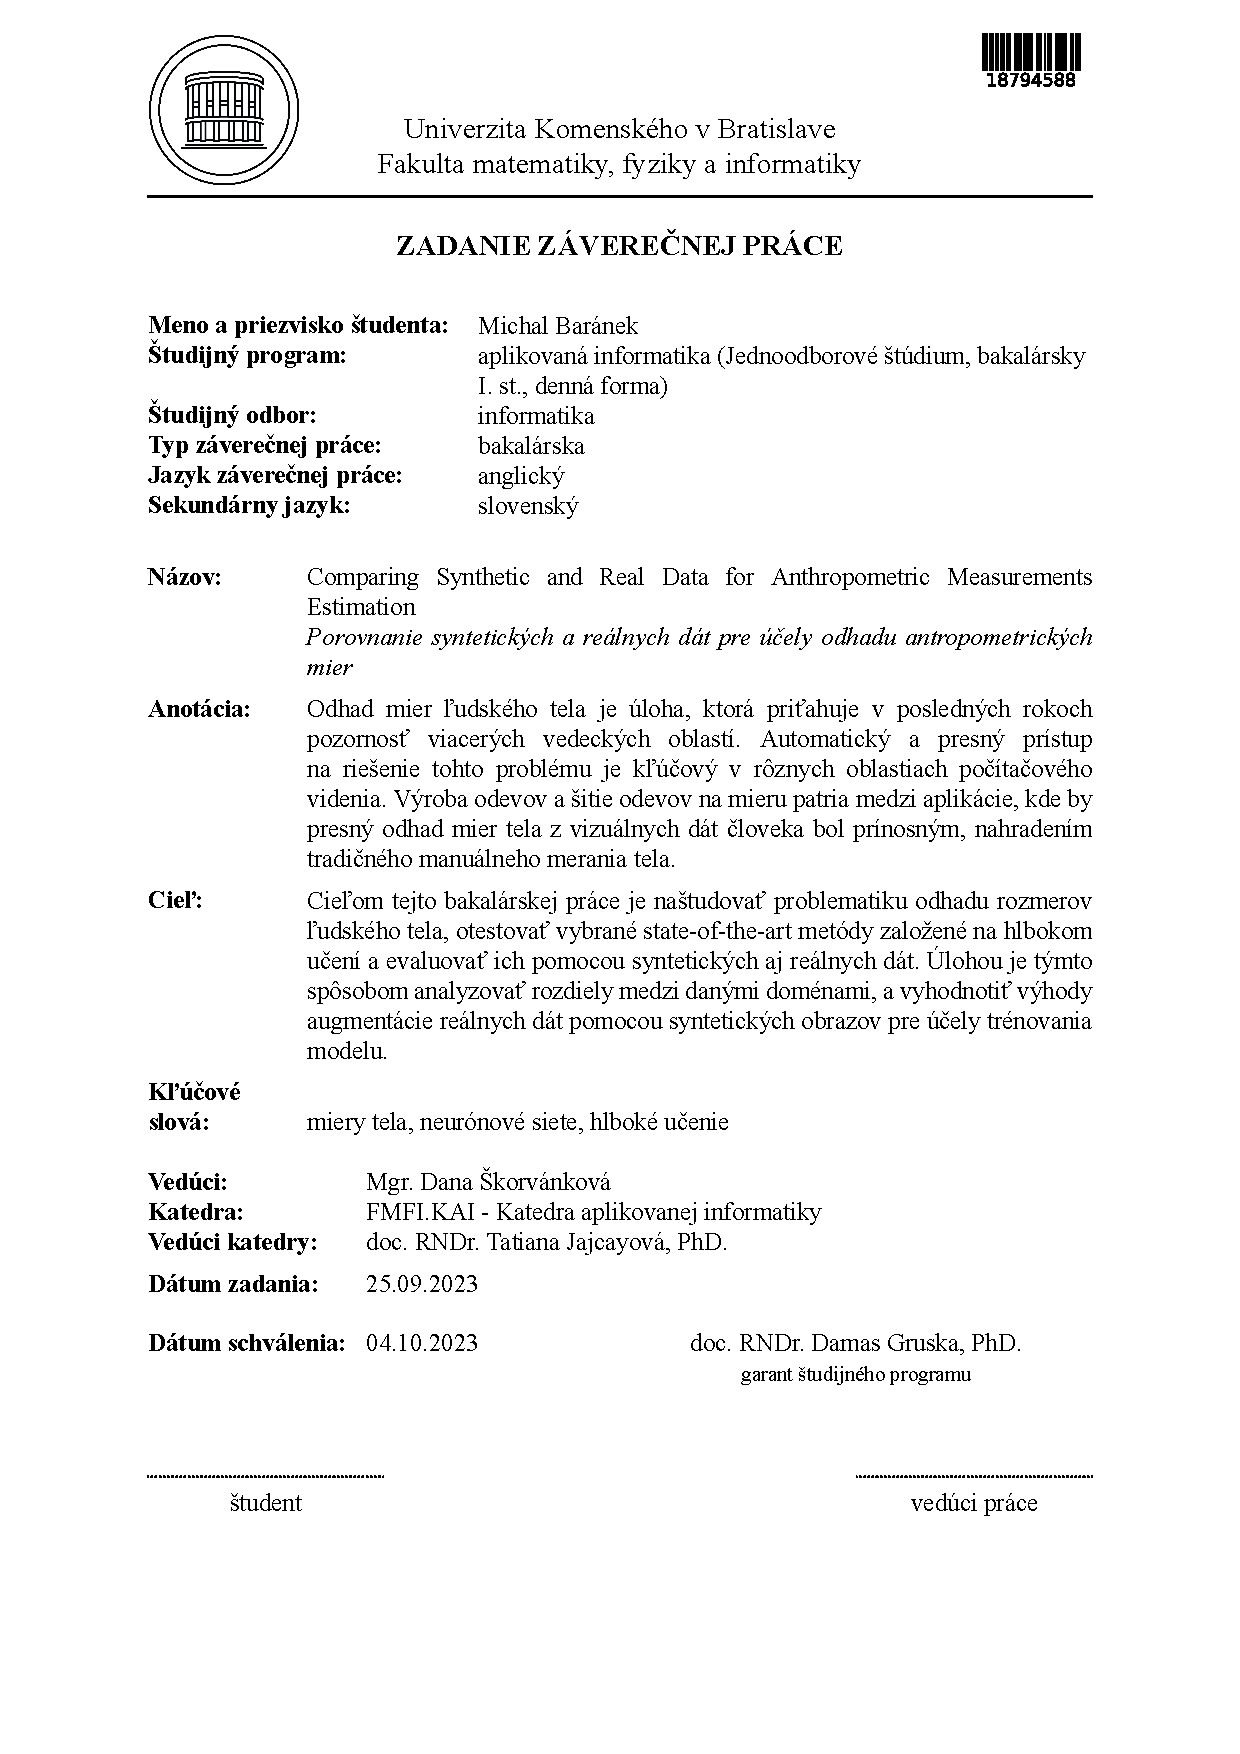
\includepdf{images/zadanie.pdf}

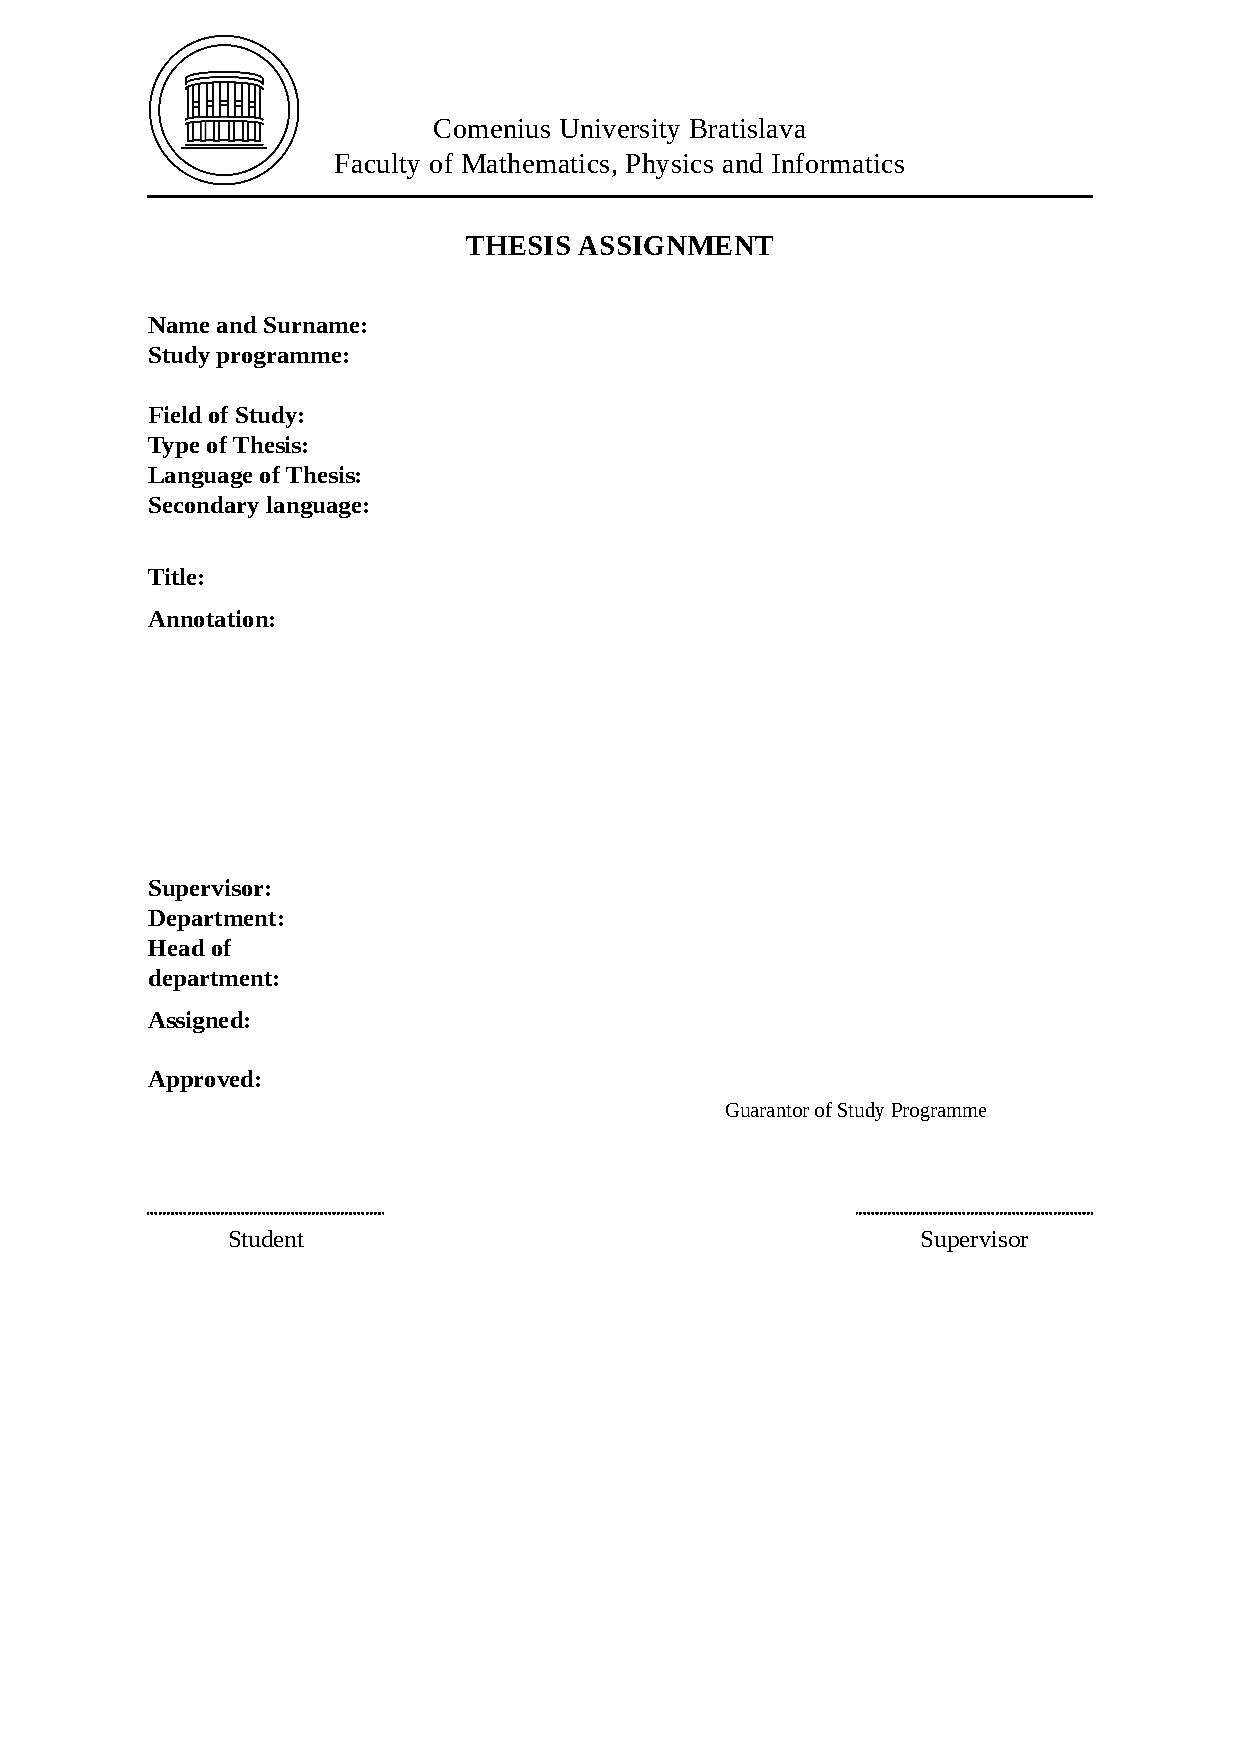
\includepdf{images/zadanie-en.pdf}

% --- Koniec zadania


% -------------------
%   Poďakovanie - nepovinné
% -------------------
\newpage
\pagestyle{plain}
~

\vfill
{\bf Acknowledgments:} Tu môžete poďakovať školiteľovi, prípadne
ďalším osobám, ktoré vám s prácou nejako pomohli, poradili,
poskytli dáta a podobne.

% --- Koniec poďakovania

% -------------------
%   Abstrakt - Slovensky
% -------------------
\newpage 
\section*{Abstrakt}


Slovenský abstrakt v rozsahu 100-500 slov, jeden odstavec. Abstrakt
stručne sumarizuje výsledky práce. Mal by byť pochopiteľný pre bežného
informatika. Nemal by teda využívať skratky, termíny alebo označenie
zavedené v práci, okrem tých, ktoré sú všeobecne známe.

\paragraph*{Kľúčové slová:} jedno, druhé, tretie (prípadne štvrté, piate)
% --- Koniec Abstrakt - Slovensky


% -------------------
% --- Abstrakt - Anglicky 
% -------------------
\newpage 
\section*{Abstract}

Abstract in the English language (translation of the abstract in the
Slovak language).


\paragraph*{Keywords:} 

% --- Koniec Abstrakt - Anglicky

% -------------------
% --- Predhovor - v informatike sa zvacsa nepouziva
% -------------------
%\newpage 
%
%
%\chapter*{Preface} %
%
%Predhovor je všeobecná informácia o práci, obsahuje hlavnú charakteristiku práce 
%a okolnosti jej vzniku. Autor zdôvodní výber témy, stručne informuje o cieľoch 
%a význame práce, spomenie domáci a zahraničný kontext, komu je práca určená, 
%použité metódy, stav poznania; autor stručne charakterizuje svoj prístup a svoje
%hľadisko. 
%
% --- Koniec Predhovor


% -------------------
% --- Obsah
% -------------------

\newpage 

\tableofcontents

% ---  Koniec Obsahu

% -------------------
% --- Zoznamy tabuliek, obrázkov - nepovinne
% -------------------

\newpage 

\listoffigures
\listoftables

% ---  Koniec Zoznamov

\mainmatter
\pagestyle{headings}

%\input uvod.tex 

%\input kapitola.tex

%\input latex.tex
	
\addcontentsline{toc}{chapter}{Introduction}
\chapter*{Introduction}
Nowadays our physical bodies are not enough for us anymore. Thanks to modern technologies every day we come closer to living a new type of life. Virtual one. The beginnings were quite humble with us sharing our thoughts via text and shortly after empowering our life stories with images. Thanks to these innovations we were able to create a new type of business - online shops. Their popularity rose over the years and are now rivals to traditional ways of shopping. These new online stores however have a significant disadvantage in comparison. You cannot try the clothes on and see whether it will fit. Luckily we have already created clothing sizing system to help us choose the correct size. However to use this system one would need exact body measurements to look up correct size in the table. \\ \\
Online shops however were not the only blooming business in recent years. A new prospect has appeared only just recently and it caught attention of big companies straight away. The virtual world where we could meet our friends living anywhere in the world without having to leave our home. In this world everyone would have their own avatar that would represent them. Some virtual worlds would let you become whoever or even whatever you could possibly think of while some others decided to stick with realism. Realism sounds great, but this approach requires realistic data to be able to look convincing. To create a clone of human body in the virtual world we amongst many variables would need exact body measurements to provide a believable result.\\ \\
These are just two examples that require users to obtain their body measurements. While the act of measuring does not seem very problematic the measurements are prone to human error. There are no rules when it comes to measuring body parts. Usually, subjects are only guided via text or image showing them how to measure. This will never satisfy the accuracy that is required.\\ \\
Thanks to progress in neural networks a new way of obtaining body measurements has emerged. With requiring only picture of body from front we can train a neural network to predict measurements of human body. This has already been proven plausible, but the accuracy lacked in some measurements. The goal of this work is to compare different .... (To make data better). The methods will vary to see how impactful they are regarding the final result.\\\\
For training we will use a synthetic dataset which will allow us to have much larger number of samples for training. For metrics we will use performance on dataset with real samples provided by BodyM dataset.\\\\
The first chapter will provide overview of the problematic, will look into traditional measuring methods, delve into obstacles this approach faces and then explain some of the mechanical works of this thesis. Second chapter will look into already existing work that is relevant to topic. In the third chapter we will define datasets. Contents of fourth chapter will focus on proposed solution and implementation. Results of our research will be located in fifth chapter while the sixth chapter will provide conclusion.
\chapter{Overview}

Contents of this chapter will provide definitions and explanations to terms and methods used in following chapters. This will hopefully help to understand the topic discussed in this thesis.


\section{Measuring}
Measuring locations vary depending on the use and thus there is no universal guide. The professionals should be familiar with the measurements required in their field of application, but the subjects themselves are usually not as informed. This can then result into incorrect measurement.

Human body can be measured using different methods. These are usually dependent on input data and thus not every method can be used in every situation.  

\subsection{Hand measurement}
This is the traditional method of using tape or any alike measuring device for obtaining measurements. The approach usually needs one extra person that performs the measurement on the subject. Due to measurements requiring to be taken at specific locations to provide correct information, a person without help is more prone to obtaining incorrect measurements.


\subsection{Digital measuring on 3D model}
Another method used for obtaining measurements is by using scanning technology. One of approaches uses devices such as photogrammetry scanners creates realistic meshes of scanned subject. The data can then be registered to SMPL \cite{smpl} mesh topology. We can then use the resulting mesh for calculating the required measurements. This is also the case of \cite{BodyM}, which uses these measurements as ground truth data.
\subsubsection{Photogrammetry scanner}
This method utilises photographs from different angles and positions to calculate and create a mesh. The device to take photos does not need any extra functionality to produce images processable into final model. However, photogrammetry scanners are being developed to provide ease of use and quality over common cameras. One of such features is a multi-camera system. Main advantage is when the subject is a living being, offering photos from multiple angles in the same instant. This prevents to faulty models due to unwilling movement of the subject.
\\

Different approach uses 3D scanning devices. These are more expensive than equipment required for photogrammetry, but can provide precise models. The result of scan using a 3D scanner is a point cloud or a set of data points depicting shape and size of subject~\cite{3dScan}. This can be used directly as and input for further processing.
\subsubsection{3D scanner}
Multiple technologies are used in 3D scanners. For example structured and laser based scanners use light to measure location of points. These devices throw blue light and cameras to record the reflection to obtain distance of point on the subject from the measuring device. While laser based devices produces lines on the subject the structured light based devices project a grid


\subsection{Using point clouds}
Not all scans are registered to a mesh topology. Some approaches have tried to use point cloud representation. An overview of methods used is provided by \cite{pointcloudMultiple}. 
%WOULD NEED TO WRITE MORE







\section{SMPL}
SMPL~\cite{smpl} is short for Skinned Multi-Person Linear model. Its capabilities include generation of animated human bodies with various body shapes in specific poses. Moreover, the model is able to deform naturally. This soft-tissue motion produces results much closer to real tissue. SMPL builds on blend shapes which are represented by a vector of concatenated vertex offsets. Other than vertices the SMPL model also uses joints, which essentially create the skeleton of the model. Topology of said model does not depend on sex of resulting model.



\section{Neural network}
Neural network is code built on premises of how human brains work. It consists of connected nodes called neurons. Each neuron takes input variables, processes them and then sends the result to other neurons. Every connection has associated weight which determines the influence said value will have.
Neurons are then organised into layers. They are usually divided into input, output and hidden layers. The function of the hidden layers is to perform the operations needed to calculate output from the input data.
The process of training adjusts the weights of the connections. This automatic process of adjusting is usually based on comparing the output and correct value we provide for the network and minimising the difference.
This process helps the network to find complex relationships or patterns that may not  be as understandable for humans.

\subsubsection{Hyperparameter}
Hyperparameter is a parameter that is not learned but chosen by developer.  These parameters do not change over time. These can be - choice of optimizer, learning rate,  number of layers, filter size and more.\\\\
\subsubsection{Loss functions \cite{loss}}
The training process is guided by the loss function. They show how good or how bad the network is at predicting the output. The results then serve as a guide for the learnable parameters. Loss function measures the difference between the predicted and expected outputs. Main goal of the network then becomes to minimise the loss function. One of the commonly used losses for regression task such as this one is the mean squared error (MSE or sometimes called L2 loss). This loss function is calculated as an average of the squared difference between the predicted values and the ground truth. To define this function mathematically:
\begin{equation}
	MSE = \frac{1}{n}\sum_{i=1}^{n}(y_i -  \hat{y_i})^2
\end{equation}
In this equation $n$ is used to define number of samples, $y_i$ is the ground truth and $\hat{y_i}$ the predicted value of the $i^{th}$ sample. Being a convex function, the MSE has a unique global minimum, which helps the optimization process as the optimization methods do not get stuck in the local minima. While being a computationally simple , it is vulnerable to outliers. The issue is created by the square nature of this function. In case of existing outlier the function gets heavily influenced and may not perform as well.
\\
\subsubsection{Performance metrics}
After the network was trained on the training data, it has to face new, unseen data. This ability is then measured using performance metrics. They are mainly used after the network has been trained. Performance metrics are also used to compare different networks. We can use some loss functions for performance metrics. In this thesis we will use mean absolute error (MAE or L1 loss). The principle is similar to MSE, but instead of squaring the difference we will use the absolute value to always have error larger than 0, meaning 0 will be a perfect fit. Mathematical definition of the MAE is as follows:
\begin{equation}
	MAE = \frac{1}{n}\sum_{i=1}^{n}|y_i -  \hat{y_i}|,
\end{equation}
in which $n$ is used to define number of samples, $y_i$ is the ground truth and $\hat{y_i}$ the predicted value of the $i^{th}$ sample.

\subsubsection{Overfitting}
One of the dangers of using neural networks is the possibility of overfitting. This issue is created when a complex network is trained with insufficient data. Complexity of architecture helps the network to find and learn more complex relationships, but in a case when inadequate amount of data is used for training, the network does not find the relationships we want, but instead learns exact values to have the best results for provided images. Consequence of this issue is, that the training loss is extremely small, but the performance metrics show inadequately larger error.
\\\\

Our model is mainly built on the following layers:

\subsubsection{Convolution layer}
Most popularly used with convolutional neural networks \cite{convolutional} this layer plays important role in network's functionality. It is based on working with matrices called kernels.  The values in kernel are learnable, which means they are adjusted over the training process to enhance performance. In this thesis we will be using these hyperparameters:
\begin{itemize}
	\item \textbf{Depth} determines dimension of the output volume (activation maps). Influences pattern recognition as well as number of neurons.
	\item \textbf{Size} determines dimensions of kernel.
	\item \textbf{Activation function}
\end{itemize}
The algorithm consists of sliding kernel along the input. At every position it calculates the sum of element-wise multiplication of corresponding pixels in input and kernel. The result is then inserted into the output. This process is then repeated over the whole input multiple times (depending upon number of kernels) %CHECK THIS WHOLE PART PLEASE 
Result of this operation captures local patterns while preserving positional relationships.


\subsubsection{Max Pooling layer}
Max pooling is an operation of non-linear down-sampling. This means that the output image of this layer is usually smaller than the input. This helps to reduce parameters for next convolutional layer, providing faster training.  This layer is defined by two hyperparameters:

\begin{itemize}
	\item \textbf{Filter size} determines the dimensions. In case of the filter reaching out of the array, only valid values are taken into consideration.
	\item \textbf{Stride} determines how many columns will the filter move.
\end{itemize}

The higher these hyperparameters' values are the smaller will the output be.\\
%CHECK IF FIELD IS THE CORRECT TERM
This layer iterates over input field and looks at subfield with size of filter size. In this subfield it finds the largest number and writes only the largest number into the output field. After this, the filter moves by stride columns left until all columns were checked. In that case the filter moves back to first column of the input field and then moves down by the stride (refer to \ref{maxPooling} as an example).\\ This process is repeated until whole input field is iterated.

\begin{figure}
	\centering{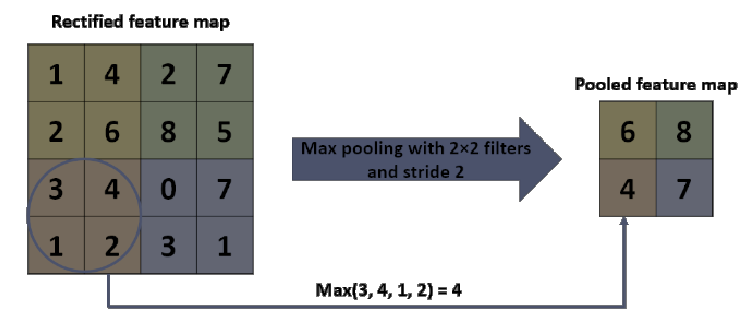
\includegraphics[scale=0.4]{images/MaxPoolingExample}}
	\caption[Max Pooling Example]{Max Pooling Example \cite{pooling}}
	\label{maxPooling}
\end{figure}

\section{Used software}
\subsubsection{Keras \cite{keras}}
Keras is an open-source neural network library written in Python. Thanks to its user-friendly interface and modular design is Keras one of the leading frameworks in neural network development. Its simple yet flexible architecture allows for easy prototyping and experimentation, making it an ideal choice for both beginners and experienced practitioners in the field of deep learning.
\subsubsection{OpenCV \cite{opencv}}
Open Source Computer Vision Library (OpenCV for short) is a comprehensive open-source library originally developed by Intel. It is mainly used for various tasks in fields such as computer vision or machine learning. In the time of writing this thesis, OpenCV provides over 2500 optimized algorithms. These are able to effectively perform many tasks such as face detection, object tracking, image preprocessing and many more. Providing interfaces in multiple programming languages such as Python, C++, Java and MATLAB it is very popular with community as well as recognisable and famous companies.%Add reference?


%\begin{figure}
%	%vlozenie samotneho obrazku vycentrovaneho a vhodnej velkosti
%	%obrazok je v subore images/cervik.png
%	\centering{\includesvg[scale=0.7]{images/DatasetComparation}}
%	%popis obrazku
%	\caption[Ukážka hry Červík]{Ukážka hry Červík. Červík je znázornený červenou farbou, voľné políčka sivou, jedlo zelenou a steny čiernou. Hoci tento popis obrázku je dlhší, v zdrojovom texte je aj kratšia verzia, ktorá sa zobrazí v zozname obrázkov.}
%	%id obrazku, pomocou ktoreho sa budeme na obrazok odvolavat
%	\label{fig:beep}
%\end{figure}\includegraphics
\chapter{Related Work}
\section{Super()}
\section{Adversarial Body Sim}
\section{Suggested approach}
\chapter{Dataset overview}
\section{Surreact}
\subsection{Description}
\subsection{SMPL}
\section{BodyM}
\subsection{Overview}
\section{Implementation}




%The output tensor is then passed through ReLU~\cite{relu} along with batch optimization. Subsequently, a max pooling layer is used followed by a  convolutional layer. The output is then once again processed by max pooling layer with configuration same as before.  The result is then flattened to a tensor which is passed to a fully connected layer and a ReLU. As the last layer a regressor is used to provide the measurements estimation.


%\section{Setting up network}
%\section{Figuring out measurements}
%\section{Optimalizations}
%\subsection{Including BodyM in training}
%\subsection{Adding height}
%\subsection{Adding lateral image}
%\subsection{Combinations}


\chapter{Results}
\chapter{Conclusion}

%\input zaver.tex

% -------------------
% --- Bibliografia
% -------------------


\newpage	

\backmatter

\thispagestyle{empty}
\clearpage

\bibliographystyle{plain}
\bibliography{literatura} 

%Prípadne môžete napísať literatúru priamo tu
%\begin{thebibliography}{5}
 
%\bibitem{br1} MOLINA H. G. - ULLMAN J. D. - WIDOM J., 2002, Database Systems, Upper Saddle River : Prentice-Hall, 2002, 1119 s., Pearson International edition, 0-13-098043-9

%\bibitem{br2} MOLINA H. G. - ULLMAN J. D. - WIDOM J., 2000 , Databasse System implementation, New Jersey : Prentice-Hall, 2000, 653s., ???

%\bibitem{br3} ULLMAN J. D. - WIDOM J., 1997, A First Course in Database Systems, New Jersey : Prentice-Hall, 1997, 470s., 

%\bibitem{br4} PREFUSE, 2007, The Prefuse visualization toolkit,  [online] Dostupné na internete: <http://prefuse.org/>

%\bibitem{br5} PREFUSE Forum, Sourceforge - Prefuse Forum,  [online] Dostupné na internete: <http://sourceforge.net/projects/prefuse/>

%\end{thebibliography}

%---koniec Referencii

% -------------------
%--- Prilohy---
% -------------------

%Nepovinná časť prílohy obsahuje materiály, ktoré neboli zaradené priamo  do textu. Každá príloha sa začína na novej strane.
%Zoznam príloh je súčasťou obsahu.
%
%\input appendixA.tex

%\input appendixB.tex

\end{document}






